%!TEX root = ../thesis.tex
%*******************************************************************************
%*********************************** First Chapter *****************************
%*******************************************************************************

\chapter{Introduction}  %Title of the First Chapter

\ifpdf
    \graphicspath{{Chapter1/Figs/Raster/}{Chapter1/Figs/PDF/}{Chapter1/Figs/}}
\else
    \graphicspath{{Chapter1/Figs/Vector/}{Chapter1/Figs/}}
\fi
\section{Background}
Climate change is a well known problem among scientist since longtime, the first paper warning the effects of the increment of carbon dioxide in the athomosfhere is from 1976 \cite{manabe_thermal_1967} while in a study of 1976 \cite{keeling_atmospheric_1976} they observed it for the first time. In 1988 the World Meteorological Organization Established the Intergovernmental Panel On Climate Change (IPCC) \cite{baker_1989} which is up to know the main organization evaluating climate change. As showed in \cite{santos_climate_2021} the researcher interest in climate change startes growing significantly after 1990. 

\begin{figure}[H]
    \centering
    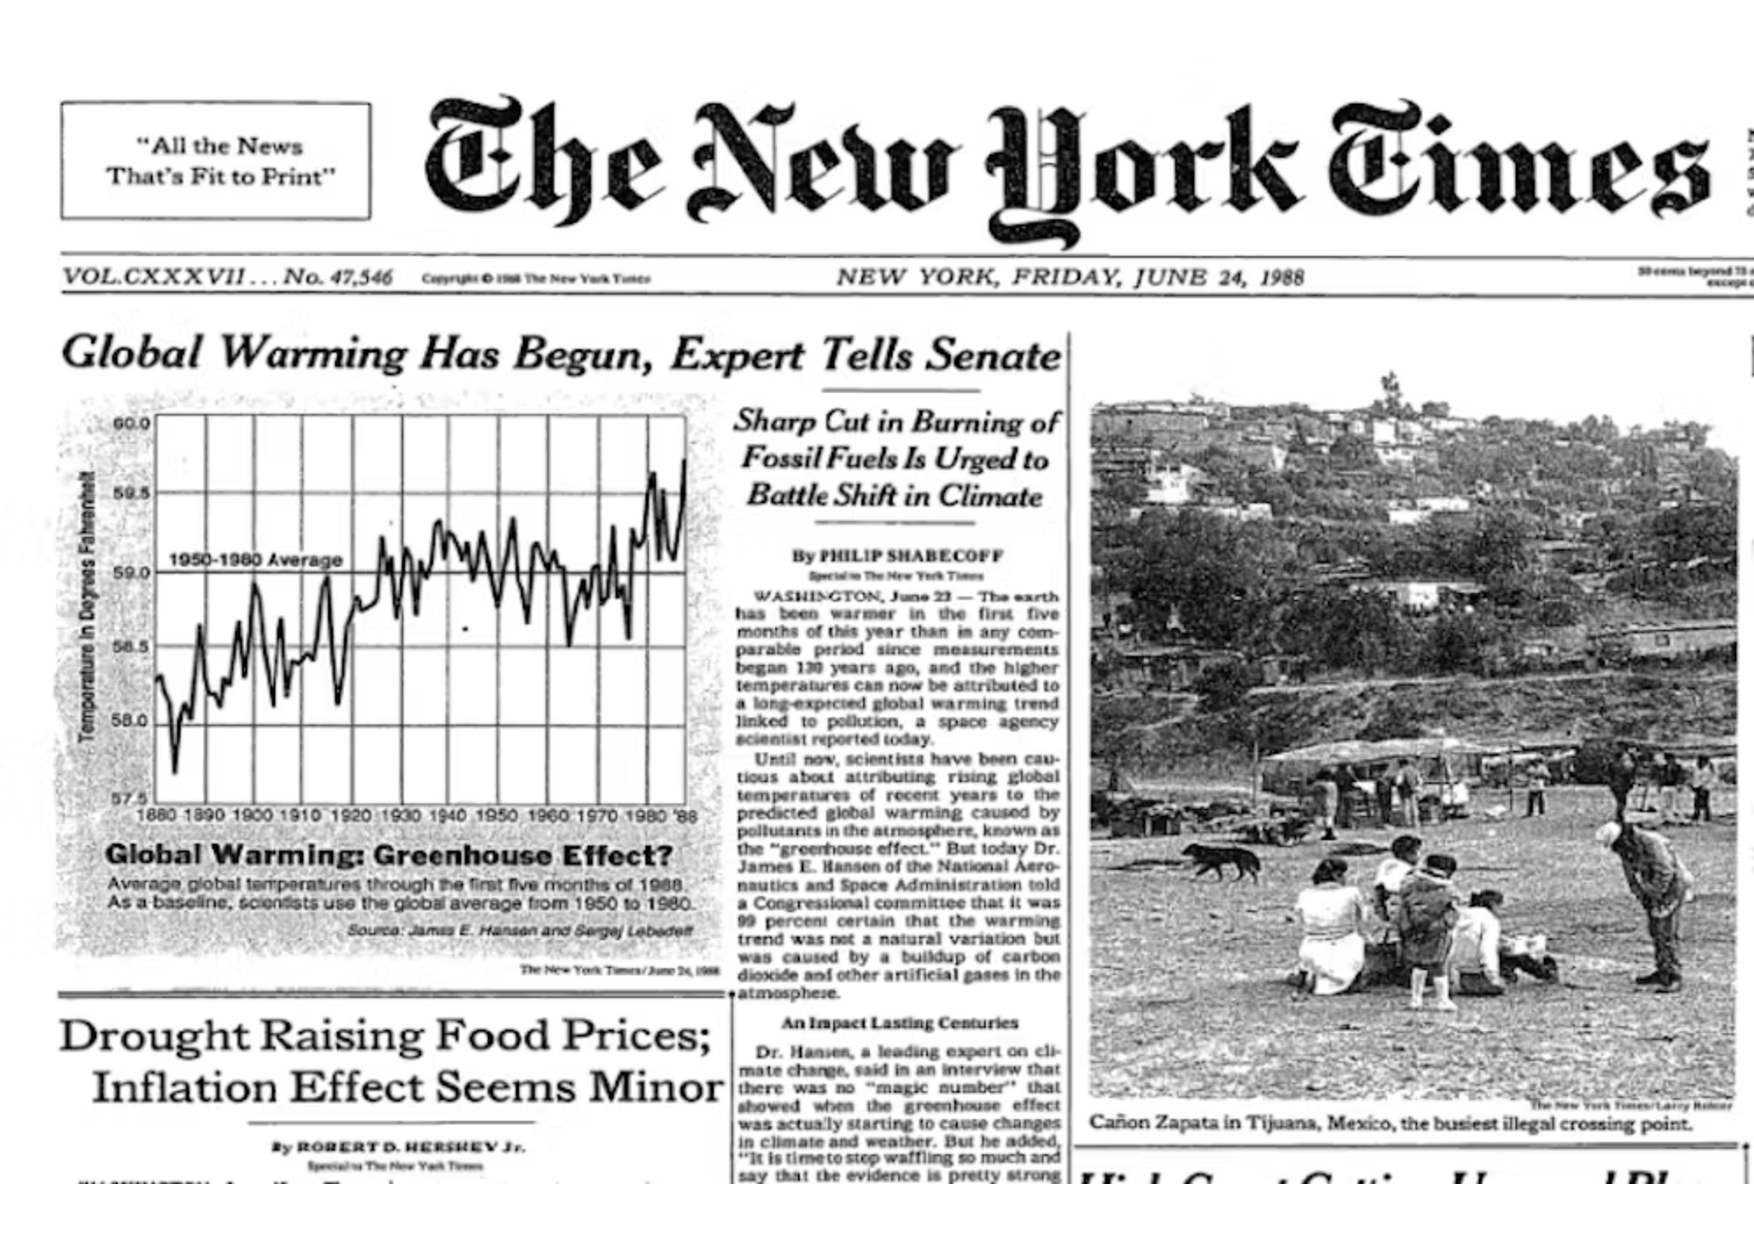
\includegraphics[width=0.75\linewidth]{Chapter1/figures/global_warming copy.pdf}
    \caption{Front page of NY times, June 24 1988 }
    \label{fig:enter-label}
\end{figure}

Only in the past few years has become mainstream, in part thanks to Greta Thunberg \cite{sabherwal_greta_2021} and Fridays for Future people were more aware of the problem. As we can see in Fig \ref{fig:google_greta} only after 2019 people started searching (and talking) about a climate crisis, underlining  the urgency with which we should act. It is also true that the strikes caused inconvenience to many normal citizen trying to go to their workplace. This mean that someone may have developed a bad feeling towards this activism and thus towards climate change. In fact an increase in polarization have been detected after the strikes \cite{Falkenberg_climate_2022}.
\\


\begin{figure}
    \centering
    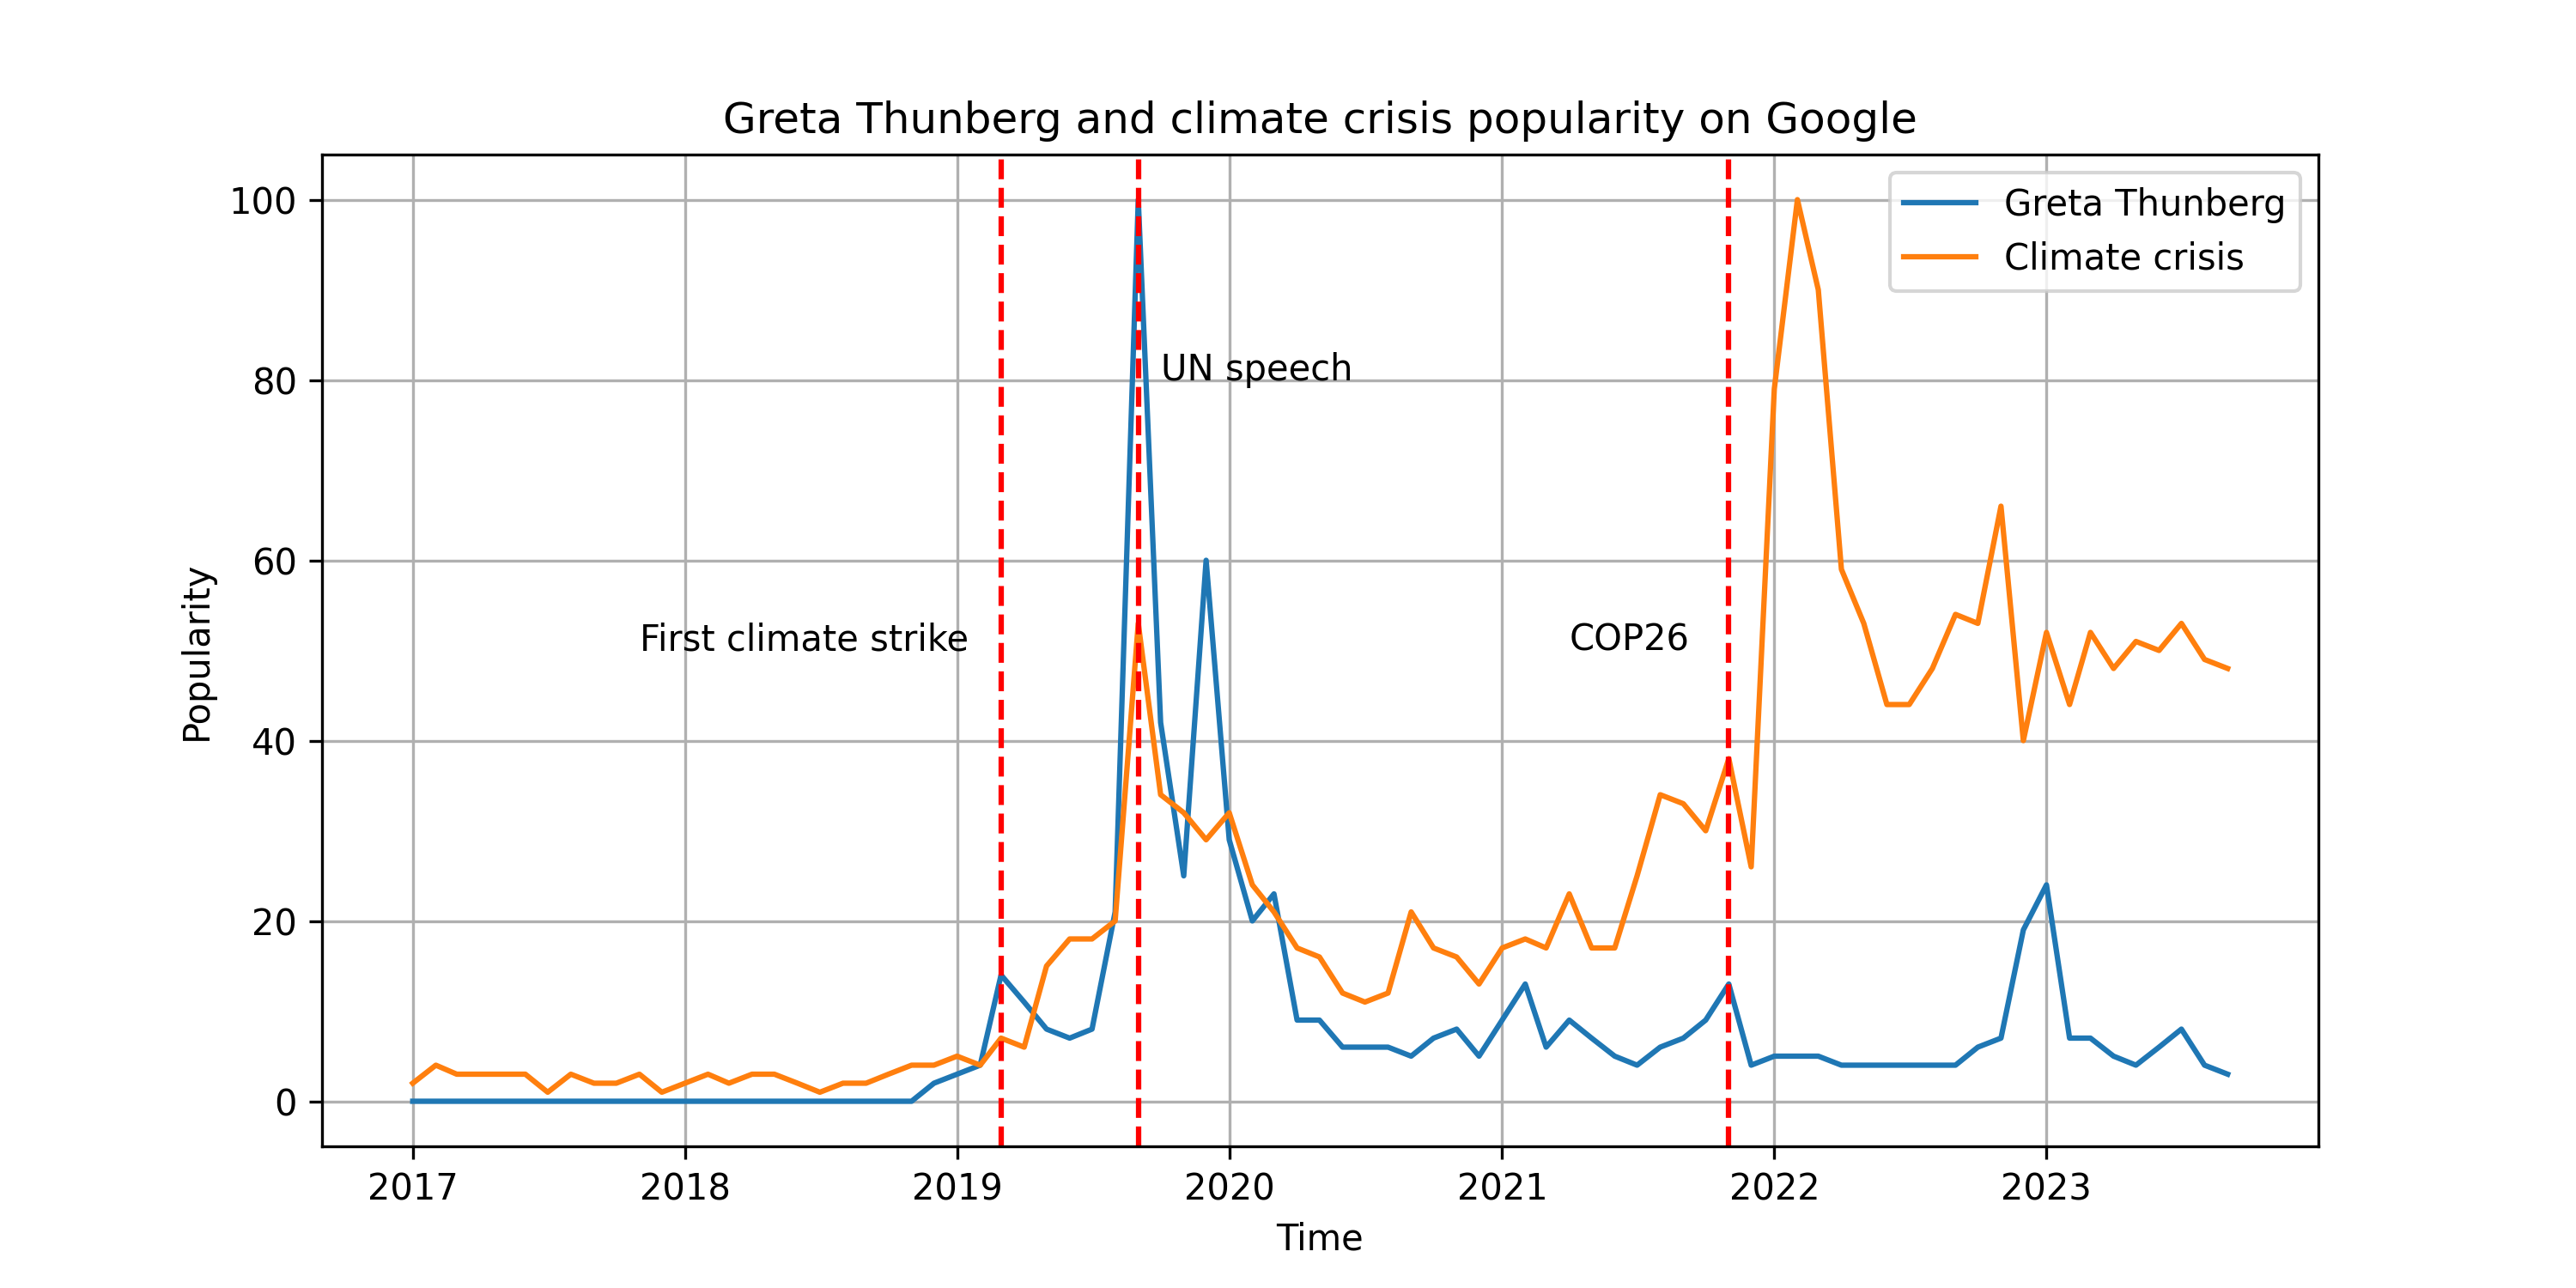
\includegraphics[width=0.85\linewidth]{Chapter1/figures/greta_climate_crisis.png}
    \caption{Interest on google over the time of Greta Thunberg and climat crisis}
    \label{fig:google_greta}
\end{figure}
In particular twitter is a place where political debate take place \cite{Pew_twitter_2022}, and political events like 
Conference of Parties (COP) are the perfect opportunity to study the climate change discussion because are the conferences where the highest political figures of many countries meet and talk about the climate emergencies. 



\paragraph{Conference of Parties}
Conferences of Parties are yearly conferences organized by United Nations where the topic of discussion is climate change, the first has been held in 1995 in Berlin, the ones that ended with a document to ratify are:
\begin{itemize}
    \item \textbf{COP3}: Kyoto protocol (1997) It was the first treaty to legally mandate countries to cut down on greenhouse gas emissions, but this was true only for developed countries, so excluding china and india.
    \item \textbf{COP21}: The Paris Agreement is a global accord that aims to limit global warming to well below 2 degrees Celsius, preferably to 1.5 degrees Celsius, compared to pre-industrial levels by requiring all countries to set their own emissions reduction targets. It is considered more effective and inclusive than the Kyoto Protocol because it involves all countries, allows for flexibility in setting emissions targets, and includes a robust system for transparency and accountability.
    \item \textbf{COP26}: Glasgow Climate Pact (2021) is a crucial agreement in the global effort to combat climate change. It includes significant commitments to address the urgent challenges of climate change, such as phasing down coal usage, increasing climate finance for adaptation, strengthening international cooperation, and supporting countries in transitioning to low-carbon economies. But not everyone agrees that that they did a good job \cite{arora_cop26_2021} \cite{layna_promises_2022} \cite{suresh_climate_2021}
\end{itemize}

\\

For the first one unfortunatly we do not have twitter data but for the latter two we have, and our focus will be on that two .

In particular we will study the well known phenomenon among social scientist of polarization of which we do not have a universally agreed definition, in this paper we will use the one stated in \cite{bramson_understanding_2017}: “the most common measure of polarization in the political literature is probably bimodality, which is the idea that the population can be usefully broken down into two subpopulations”\\




This work lays its foundations on the research of Falkenberg et al \cite{falkenberg_growing_2022} where they discovered that the cop26 was way more polarized then cop21. Using a similar approach we will explore the ideological polarization topic by topic. 


\section{Research Questions}
Thanks to the structure we gave to our research we can now answer a new set of questions, related to the intratopic polarization, the first and most straightforward is RQ1 that has the goal to inspect the topics that are driving the polarization of the entire COP26. Consequently RQ2 wants to identify if these topics have always been so polarized or not.

Then we will move to some questions related to the users, in particular RQ3 want to see if the polarized users are polarized in the same way over the different topics or if there are topics in which they are in the opposite side of the spectrum. RQ4 instead investigate whether the users that talks about many different topics are more polarized than the user that are present in only one.



\begin{enumerate}
    \item  Which are the most polarizing topics discussed on twitter during cop 26?
    \item how did topics evolved between cop21 and cop26?
    \item Is the single user polarization different across different topics? ( quelli a destra stanno  a destra in tutti i topic?)
    \item Are the users present in more topics polarized in different ways that the ‘experts’ that are present only in one or few topics?

\end{enumerate}






%********************************** %First Section  **************************************

\nomenclature[z-DEM]{DEM}{Discrete Element Method}
